\begin{figure}[h!]
	\centering
	
	
	\tikzset{every picture/.style={line width=0.75pt}} %set default line width to 0.75pt        
	
	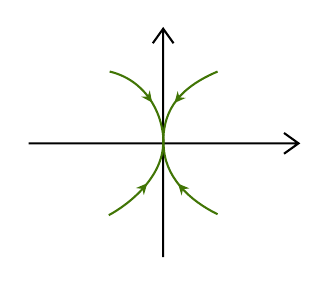
\begin{tikzpicture}[x=0.75pt,y=0.75pt,yscale=-1,xscale=1]
		%uncomment if require: \path (0,300); %set diagram left start at 0, and has height of 300
		
		%Shape: Axis 2D [id:dp9380995091348139] 
		\draw  (130,135.23) -- (260,135.23)(194.78,80) -- (194.78,190) (253,130.23) -- (260,135.23) -- (253,140.23) (189.78,87) -- (194.78,80) -- (199.78,87)  ;
		%Curve Lines [id:da7464742185837894] 
		\draw [color={rgb, 255:red, 65; green, 117; blue, 5 }  ,draw opacity=1 ]   (194.78,135.23) .. controls (194.78,122.17) and (199.33,109.79) .. (221,100.63) ;
		\draw [shift={(200.24,115.76)}, rotate = 310.45] [fill={rgb, 255:red, 65; green, 117; blue, 5 }  ,fill opacity=1 ][line width=0.08]  [draw opacity=0] (5.36,-2.57) -- (0,0) -- (5.36,2.57) -- (3.56,0) -- cycle    ;
		%Curve Lines [id:da3247666901842563] 
		\draw [color={rgb, 255:red, 65; green, 117; blue, 5 }  ,draw opacity=1 ]   (168.57,169.83) .. controls (178.33,164.67) and (194.57,151.5) .. (194.78,135.23) ;
		\draw [shift={(187.11,154.49)}, rotate = 131.69] [fill={rgb, 255:red, 65; green, 117; blue, 5 }  ,fill opacity=1 ][line width=0.08]  [draw opacity=0] (5.36,-2.57) -- (0,0) -- (5.36,2.57) -- (3.56,0) -- cycle    ;
		%Curve Lines [id:da34070001099076586] 
		\draw [color={rgb, 255:red, 65; green, 117; blue, 5 }  ,draw opacity=1 ]   (221,169.38) .. controls (207.78,162.96) and (194.78,151.27) .. (195,135) ;
		\draw [shift={(201.96,154.66)}, rotate = 47.94] [fill={rgb, 255:red, 65; green, 117; blue, 5 }  ,fill opacity=1 ][line width=0.08]  [draw opacity=0] (5.36,-2.57) -- (0,0) -- (5.36,2.57) -- (3.56,0) -- cycle    ;
		%Curve Lines [id:da12862086047130106] 
		\draw [color={rgb, 255:red, 65; green, 117; blue, 5 }  ,draw opacity=1 ]   (195,135) .. controls (194.57,118.96) and (185.25,104.52) .. (169,100.63) ;
		\draw [shift={(189.43,115.52)}, rotate = 233.71] [fill={rgb, 255:red, 65; green, 117; blue, 5 }  ,fill opacity=1 ][line width=0.08]  [draw opacity=0] (5.36,-2.57) -- (0,0) -- (5.36,2.57) -- (3.56,0) -- cycle    ;
		
		
		
		
	\end{tikzpicture}
	
	
\end{figure}